% figures/embedders.pdf, its alt text and tables/recipes.tex are generated by benchmarks/scripts/results and copied by benchmarks/scripts/copy.sh
\begin{figure*}[t]
\centering
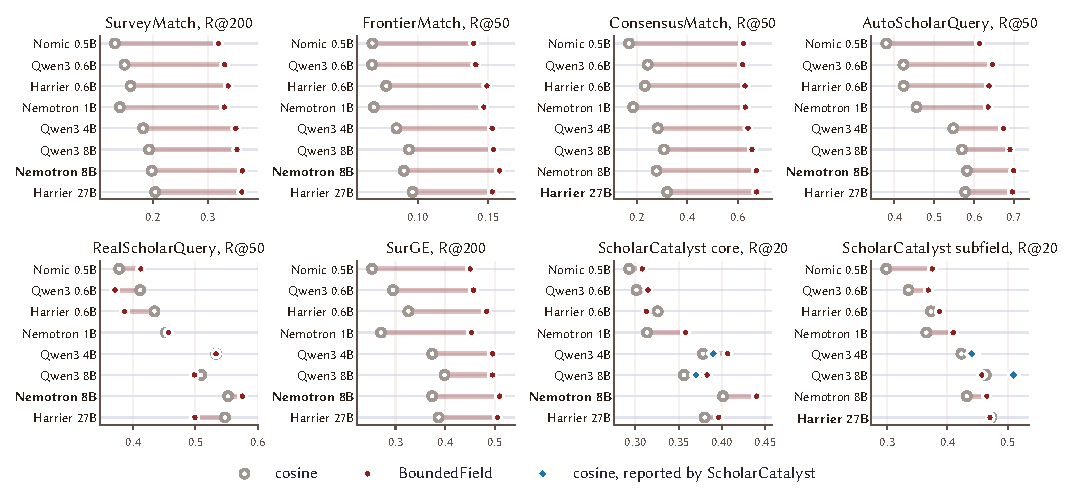
\includegraphics[width=\textwidth]{figures/embedders.pdf}
\Description{Eight dot-line panels in two rows, one per benchmark, each listing eight embedders from top to bottom by size: Nomic 0.5B, Qwen3 0.6B, Harrier 0.6B, Nemotron 1B, Qwen3 4B, Qwen3 8B, Nemotron 8B, Harrier 27B. Each row joins a hollow gray dot, recall with cosine search, an amber dot, recall with PPR, and a red dot, recall with BoundedField, and the embedder with the highest BoundedField recall in each panel is in bold. A star beside an embedder marks BoundedField significantly above its cosine search and a cross significantly above its PPR. On SurveyMatch, FrontierMatch, ConsensusMatch, AutoScholarQuery, SurGE, every BoundedField dot sits right of every cosine dot. On the two ScholarCatalyst panels, blue diamonds mark the cosine recall ScholarCatalyst reported for Qwen3 4B and 8B. Values, cosine to PPR to BoundedField, are: SurveyMatch at R@200: Nomic 0.5B 0.132 to 0.232 to 0.319; Qwen3 0.6B 0.149 to 0.249 to 0.331; Harrier 0.6B 0.160 to 0.252 to 0.337; Nemotron 1B 0.141 to 0.240 to 0.330; Qwen3 4B 0.183 to 0.278 to 0.350; Qwen3 8B 0.194 to 0.284 to 0.353; Nemotron 8B 0.198 to 0.295 to 0.363; Harrier 27B 0.205 to 0.290 to 0.361; best with BoundedField, Nemotron 8B. FrontierMatch at R@50: Nomic 0.5B 0.068 to 0.078 to 0.142; Qwen3 0.6B 0.068 to 0.079 to 0.139; Harrier 0.6B 0.078 to 0.089 to 0.145; Nemotron 1B 0.069 to 0.079 to 0.146; Qwen3 4B 0.085 to 0.097 to 0.152; Qwen3 8B 0.094 to 0.103 to 0.155; Nemotron 8B 0.090 to 0.099 to 0.159; Harrier 27B 0.096 to 0.094 to 0.153; best with BoundedField, Nemotron 8B. ConsensusMatch at R@50: Nomic 0.5B 0.170 to 0.470 to 0.607; Qwen3 0.6B 0.243 to 0.504 to 0.628; Harrier 0.6B 0.232 to 0.509 to 0.635; Nemotron 1B 0.185 to 0.502 to 0.627; Qwen3 4B 0.283 to 0.572 to 0.651; Qwen3 8B 0.308 to 0.599 to 0.662; Nemotron 8B 0.278 to 0.597 to 0.663; Harrier 27B 0.321 to 0.588 to 0.673; best with BoundedField, Harrier 27B. AutoScholarQuery at R@50: Nomic 0.5B 0.379 to 0.482 to 0.621; Qwen3 0.6B 0.423 to 0.527 to 0.646; Harrier 0.6B 0.423 to 0.521 to 0.641; Nemotron 1B 0.455 to 0.557 to 0.639; Qwen3 4B 0.548 to 0.632 to 0.690; Qwen3 8B 0.569 to 0.630 to 0.691; Nemotron 8B 0.582 to 0.663 to 0.702; Harrier 27B 0.578 to 0.634 to 0.694; best with BoundedField, Nemotron 8B. RealScholarQuery at R@50: Nomic 0.5B 0.377 to 0.404 to 0.374; Qwen3 0.6B 0.411 to 0.414 to 0.404; Harrier 0.6B 0.434 to 0.445 to 0.381; Nemotron 1B 0.453 to 0.444 to 0.425; Qwen3 4B 0.533 to 0.516 to 0.470; Qwen3 8B 0.509 to 0.499 to 0.493; Nemotron 8B 0.553 to 0.516 to 0.574; Harrier 27B 0.547 to 0.530 to 0.470; best with BoundedField, Nemotron 8B. SurGE at R@200: Nomic 0.5B 0.253 to 0.391 to 0.450; Qwen3 0.6B 0.295 to 0.405 to 0.458; Harrier 0.6B 0.326 to 0.425 to 0.479; Nemotron 1B 0.271 to 0.368 to 0.453; Qwen3 4B 0.374 to 0.453 to 0.487; Qwen3 8B 0.399 to 0.457 to 0.502; Nemotron 8B 0.374 to 0.475 to 0.508; Harrier 27B 0.387 to 0.453 to 0.507; best with BoundedField, Nemotron 8B. ScholarCatalyst core at R@20: Nomic 0.5B 0.293 to 0.304 to 0.289; Qwen3 0.6B 0.301 to 0.341 to 0.321; Harrier 0.6B 0.326 to 0.339 to 0.315; Nemotron 1B 0.314 to 0.333 to 0.326; Qwen3 4B 0.378 to 0.378 to 0.386; Qwen3 8B 0.356 to 0.377 to 0.375; Nemotron 8B 0.401 to 0.371 to 0.436; Harrier 27B 0.380 to 0.399 to 0.385; best with BoundedField, Nemotron 8B; reported cosine 0.39 for Qwen3 4B; reported cosine 0.37 for Qwen3 8B. ScholarCatalyst subfield at R@20: Nomic 0.5B 0.298 to 0.330 to 0.358; Qwen3 0.6B 0.335 to 0.370 to 0.387; Harrier 0.6B 0.373 to 0.405 to 0.377; Nemotron 1B 0.365 to 0.385 to 0.393; Qwen3 4B 0.423 to 0.442 to 0.432; Qwen3 8B 0.464 to 0.487 to 0.452; Nemotron 8B 0.432 to 0.431 to 0.466; Harrier 27B 0.473 to 0.492 to 0.463; best with BoundedField, Nemotron 8B; reported cosine 0.44 for Qwen3 4B; reported cosine 0.51 for Qwen3 8B.}

\caption{R@$k$ with cosine search, PPR, and BoundedField by embedder on all benchmarks, at each benchmark's middle cutoff. BoundedField runs used the recipe of each benchmark's mode, refit on each embedder: \term{survey} on SurveyMatch and SurGE, \term{frontier} and \term{consensus} on their own, and \term{focused} on PaSa and ScholarCatalyst. The embedding in bold has the highest BoundedField score. A star beside an embedder marks BoundedField significantly above its cosine search, and a cross significantly above its PPR, by a one-sided Wilcoxon signed-rank test on per-case recall, Holm-corrected over the 64 comparisons of each, $p < 0.05$. Diamond marks the cosine recall reported by ScholarCatalyst \cite{kim2026scholarcatalyst}.}
\label{fig:embedders}
\end{figure*}

% generated by benchmarks/scripts/results/table_main_recipes.py from benchmarks/data/runs/tune/nomic-focused_bf_seed0, benchmarks/data/runs/tune/nomic-survey_bf_seed0, benchmarks/data/runs/tune/nomic-frontier_bf_seed0, benchmarks/data/runs/tune/nomic-consensus_bf_seed0
\begin{table}[t]
\caption{The exponents of BoundedField's four recipes, with the benchmark and the R@$k$ each was tuned on.}
\label{tab:recipes}
\centering
\small
\setlength{\tabcolsep}{4pt}
\begin{tabular}{lrrrr}
\toprule
 & \term{focused} & \term{survey} & \term{frontier} & \term{consensus} \\
\midrule
\textbf{Source} & PaSa & SurveyMatch & FrontierMatch & ConsensusMatch \\
$k$ & 20 & 250 & 100 & 50 \\
\midrule
$w_{\text{cos}}$ & 1.00 & 1.00 & 1.00 & 1.00 \\
$w_{\text{rec}}$ & 0.45 & 0.95 & 0.85 & 1.59 \\
$w_{\text{bm25}}$ & 0.97 & 0.53 & 0.20 & 0.64 \\
$w_{\text{anc}}$ & 0.52 & 1.33 & 0.32 & 2.72 \\
$w_{\text{fro}}$ & 0.01 & 0.23 & 0.27 & 0.02 \\
$w_{\text{anc2}}$ & 0.13 & 0.26 & 0.00 & 0.08 \\
$w_{\text{fro2}}$ & 0.01 & 0.03 & 0.02 & 0.02 \\
$w_{\text{cocite}}$ & 0.50 & 1.98 & 1.35 & 0.19 \\
$w_{\text{couple}}$ & 0.06 & 0.02 & 0.01 & 0.02 \\
$w_{\text{anc\_decay}}$ & 0.01 & 0.02 & 0.05 & 0.06 \\
$w_{\text{fro\_decay}}$ & 0.01 & 0.02 & 0.01 & 0.02 \\
$w_{\text{hub}}$ & 0.01 & 0.23 & 4.23 & 0.06 \\
\bottomrule
\end{tabular}
\end{table}


% generated by paper/scripts/retrieval.py
% recall is recomputed from each run's rankings against benchmarks/data/cases/<benchmark>/<split>.jsonl, and ScholarCatalyst's nDCG and recall are the means of each run's per-case values
\begin{table*}[t]
\centering
\footnotesize
\setlength{\tabcolsep}{4pt}
\begin{subtable}{\textwidth}
\centering
\caption{The proposed benchmarks, test splits.}
\label{tab:proposed}
\begin{tabular}{lrrrrrrrrr}
\toprule
 & \multicolumn{3}{c}{SurveyMatch} & \multicolumn{3}{c}{FrontierMatch} & \multicolumn{3}{c}{ConsensusMatch} \\
\cmidrule(lr){2-4}\cmidrule(lr){5-7}\cmidrule(lr){8-10}
method & R@100 & R@200 & R@500 & R@20 & R@50 & R@100 & R@20 & R@50 & R@100 \\
\midrule
% benchmarks/data/runs/bm25-surveymatch.jsonl, benchmarks/data/runs/bm25-frontiermatch.jsonl, benchmarks/data/runs/bm25-consensusmatch.jsonl
BM25 & 0.066 & 0.100 & 0.162 & 0.027 & 0.051 & 0.080 & 0.058 & 0.113 & 0.167 \\
% benchmarks/data/runs/specter2-surveymatch.jsonl, benchmarks/data/runs/specter2-frontiermatch.jsonl, benchmarks/data/runs/specter2-consensusmatch.jsonl
SPECTER2 & 0.037 & 0.057 & 0.097 & 0.018 & 0.038 & 0.056 & 0.037 & 0.073 & 0.120 \\
% benchmarks/data/runs/scincl-surveymatch.jsonl, benchmarks/data/runs/scincl-frontiermatch.jsonl, benchmarks/data/runs/scincl-consensusmatch.jsonl
SciNCL & 0.059 & 0.093 & 0.158 & 0.023 & 0.047 & 0.077 & 0.082 & 0.148 & 0.233 \\
% benchmarks/data/runs/nomic_cosine-surveymatch.jsonl, benchmarks/data/runs/nomic_cosine-frontiermatch.jsonl, benchmarks/data/runs/nomic_cosine-consensusmatch.jsonl
Nomic cosine & 0.087 & 0.133 & 0.212 & 0.032 & 0.069 & 0.107 & 0.096 & 0.172 & 0.257 \\
% benchmarks/data/runs/rerank-surveymatch.jsonl, benchmarks/data/runs/rerank-frontiermatch.jsonl, benchmarks/data/runs/rerank-consensusmatch.jsonl
OpenScholar rerank & 0.083 & 0.130 & 0.217 & 0.028 & 0.055 & 0.093 & 0.070 & 0.151 & 0.220 \\
% benchmarks/data/runs/gar_sim-surveymatch.jsonl, benchmarks/data/runs/gar_sim-frontiermatch.jsonl, benchmarks/data/runs/gar_sim-consensusmatch.jsonl
GAR (similarity) & 0.085 & 0.135 & 0.235 & 0.029 & 0.056 & 0.094 & 0.073 & 0.159 & 0.238 \\
% benchmarks/data/runs/gar_cite-surveymatch.jsonl, benchmarks/data/runs/gar_cite-frontiermatch.jsonl, benchmarks/data/runs/gar_cite-consensusmatch.jsonl
GAR (citations) & 0.090 & 0.147 & 0.275 & 0.030 & 0.058 & 0.099 & 0.076 & 0.167 & 0.254 \\
% benchmarks/data/runs/ppr-surveymatch.jsonl, benchmarks/data/runs/ppr-frontiermatch.jsonl, benchmarks/data/runs/ppr-consensusmatch.jsonl
PPR & 0.143 & 0.229 & 0.375 & 0.028 & 0.077 & 0.122 & 0.274 & 0.441 & 0.556 \\
\midrule
% benchmarks/data/runs/survey-surveymatch.jsonl, benchmarks/data/runs/frontier-frontiermatch.jsonl, benchmarks/data/runs/consensus-consensusmatch.jsonl
BoundedField (Nomic) & 0.216 & 0.319 & 0.475 & 0.067 & 0.139 & 0.224 & 0.441 & 0.624 & 0.731 \\
% benchmarks/data/runs/bfrefit_nemotron_8b-surveymatch.jsonl, benchmarks/data/runs/bfrefit_nemotron_8b-frontiermatch.jsonl, benchmarks/data/runs/bfrefit_nemotron_8b-consensusmatch.jsonl
BoundedField (Nemotron 8B) & \textbf{0.246} & \textbf{0.363} & \textbf{0.529} & \textbf{0.073} & \textbf{0.158} & \textbf{0.244} & \textbf{0.488} & \textbf{0.673} & \textbf{0.797} \\
\bottomrule
\end{tabular}
\end{subtable}
\vspace{6pt}
\begin{subtable}{\textwidth}
\centering
\caption{PaSa's AutoScholarQuery test split and RealScholarQuery, and SurGE. PaSa's reported runs search Google rather than our corpus.}
\label{tab:existing}
\begin{tabular}{lrrrrrrrrr}
\toprule
 & \multicolumn{3}{c}{AutoScholarQuery} & \multicolumn{3}{c}{RealScholarQuery} & \multicolumn{3}{c}{SurGE} \\
\cmidrule(lr){2-4}\cmidrule(lr){5-7}\cmidrule(lr){8-10}
method & R@20 & R@50 & R@100 & R@20 & R@50 & R@100 & R@100 & R@200 & R@500 \\
\midrule
% benchmarks/data/runs/bm25-pasa_test.jsonl, benchmarks/data/runs/bm25-pasa_real.jsonl, benchmarks/data/runs/bm25-surge.jsonl
BM25 & 0.238 & 0.313 & 0.376 & 0.169 & 0.255 & 0.317 & 0.150 & 0.192 & 0.258 \\
% benchmarks/data/runs/specter2-pasa_test.jsonl, benchmarks/data/runs/specter2-pasa_real.jsonl, benchmarks/data/runs/specter2-surge.jsonl
SPECTER2 & 0.120 & 0.177 & 0.220 & 0.101 & 0.152 & 0.226 & 0.184 & 0.245 & 0.338 \\
% benchmarks/data/runs/scincl-pasa_test.jsonl, benchmarks/data/runs/scincl-pasa_real.jsonl, benchmarks/data/runs/scincl-surge.jsonl
SciNCL & 0.118 & 0.174 & 0.225 & 0.104 & 0.181 & 0.253 & 0.180 & 0.239 & 0.337 \\
% benchmarks/data/runs/nomic_cosine-pasa_test.jsonl, benchmarks/data/runs/nomic_cosine-pasa_real.jsonl, benchmarks/data/runs/nomic_cosine-surge.jsonl
Nomic cosine & 0.278 & 0.375 & 0.439 & 0.270 & 0.377 & 0.477 & 0.199 & 0.255 & 0.347 \\
% benchmarks/data/runs/rerank-pasa_test.jsonl, benchmarks/data/runs/rerank-pasa_real.jsonl, benchmarks/data/runs/rerank-surge.jsonl
OpenScholar rerank & 0.298 & 0.387 & 0.452 & 0.241 & 0.383 & 0.488 & 0.174 & 0.233 & 0.341 \\
% benchmarks/data/runs/gar_sim-pasa_test.jsonl, benchmarks/data/runs/gar_sim-pasa_real.jsonl, benchmarks/data/runs/gar_sim-surge.jsonl
GAR (similarity) & 0.299 & 0.391 & 0.463 & 0.242 & 0.384 & 0.478 & 0.178 & 0.237 & 0.361 \\
% benchmarks/data/runs/gar_cite-pasa_test.jsonl, benchmarks/data/runs/gar_cite-pasa_real.jsonl, benchmarks/data/runs/gar_cite-surge.jsonl
GAR (citations) & 0.307 & 0.405 & 0.481 & 0.246 & 0.391 & 0.502 & 0.187 & 0.264 & 0.423 \\
% benchmarks/data/runs/ppr-pasa_test.jsonl, benchmarks/data/runs/ppr-pasa_real.jsonl, benchmarks/data/runs/ppr-surge.jsonl
PPR & 0.394 & 0.482 & 0.518 & 0.253 & 0.395 & 0.491 & 0.266 & 0.387 & 0.566 \\
\midrule
% benchmarks/data/runs/focused-pasa_test.jsonl, benchmarks/data/runs/focused-pasa_real.jsonl, benchmarks/data/runs/survey-surge.jsonl
BoundedField (Nomic) & 0.499 & 0.612 & 0.681 & 0.241 & 0.415 & 0.526 & 0.354 & 0.451 & 0.607 \\
% benchmarks/data/runs/bfrefit_nemotron_8b-pasa_test.jsonl, benchmarks/data/runs/bfrefit_nemotron_8b-pasa_real.jsonl, benchmarks/data/runs/bfrefit_nemotron_8b-surge.jsonl
BoundedField (Nemotron 8B) & \underline{\textbf{0.597}} & \underline{\textbf{0.699}} & \underline{\textbf{0.762}} & \textbf{0.337} & \textbf{0.576} & \textbf{0.710} & \underline{\textbf{0.394}} & \underline{\textbf{0.510}} & \underline{\textbf{0.660}} \\
\midrule
\multicolumn{10}{l}{\textit{Reported by \citet{he2025pasa}}} \\
% data/arxiv/html/2501/2501.10120.html, Table 5 (AutoScholarQuery test) and Table 6 (RealScholarQuery), Recall@20, @50, @100
Google & 0.157 & 0.189 & 0.202 & 0.183 & 0.234 & 0.254 & -- & -- & -- \\
% data/arxiv/html/2501/2501.10120.html, Table 5 (AutoScholarQuery test) and Table 6 (RealScholarQuery), Recall@20, @50, @100
Google Scholar & 0.061 & 0.097 & 0.113 & 0.151 & 0.215 & 0.281 & -- & -- & -- \\
% data/arxiv/html/2501/2501.10120.html, Table 5 (AutoScholarQuery test) and Table 6 (RealScholarQuery), Recall@20, @50, @100
Google with GPT-4o & 0.192 & 0.245 & 0.268 & 0.202 & 0.257 & 0.295 & -- & -- & -- \\
% data/arxiv/html/2501/2501.10120.html, Table 5 (AutoScholarQuery test) and Table 6 (RealScholarQuery), Recall@20, @50, @100
PaSa-7b & 0.530 & 0.633 & 0.695 & 0.580 & 0.656 & 0.693 & -- & -- & -- \\
% data/arxiv/html/2501/2501.10120.html, Table 5 (AutoScholarQuery test) and Table 6 (RealScholarQuery), Recall@20, @50, @100
PaSa-7b-ensemble & 0.533 & 0.639 & 0.710 & \underline{0.599} & \underline{0.688} & \underline{0.728} & -- & -- & -- \\
\bottomrule
\end{tabular}
\end{subtable}
\caption{Retrieval against existing methods. Every method we ran uses the Nomic embedding unless named, and BoundedField runs the recipe of each benchmark's mode: \term{survey} on SurveyMatch and SurGE, \term{frontier} and \term{consensus} on their own, and \term{focused} on PaSa and ScholarCatalyst. The Nemotron 8B row runs the same recipes refit on that embedder. Bold marks the best of our runs in each column, and an underline the best of every row, reported ones included.}
\label{tab:retrieval}
\end{table*}

\begin{table*}[t]
\ContinuedFloat
\centering
\footnotesize
\setlength{\tabcolsep}{4pt}
\begin{subtable}{\textwidth}
\centering
\caption{ScholarCatalyst, scored inside the benchmark's own corpus. Each of our cells scores every answer, then in parentheses only the answers on arXiv, as our corpus holds no other papers: 604 of the 661 core answers and 3,904 of the 4,184 subfield answers are on arXiv, and the arXiv-only score leaves out the 6 core and 5 subfield queries with none.}
\label{tab:scholarcatalyst}
\begin{tabular}{lrrrrrrrr}
\toprule
 & \multicolumn{4}{c}{core, 207 queries} & \multicolumn{4}{c}{subfield, 687 queries} \\
\cmidrule(lr){2-5}\cmidrule(lr){6-9}
method & nDCG@20 & R@5 & R@20 & R@100 & nDCG@20 & R@5 & R@20 & R@100 \\
\midrule
% benchmarks/data/runs/bm25-scholarcatalyst_core.jsonl, benchmarks/data/runs/bm25-scholarcatalyst_subfield.jsonl
BM25 & 0.170 (0.180) & 0.139 (0.150) & 0.234 (0.251) & 0.396 (0.428) & 0.213 (0.225) & 0.126 (0.139) & 0.268 (0.291) & 0.473 (0.513) \\
% benchmarks/data/runs/specter2-scholarcatalyst_core.jsonl, benchmarks/data/runs/specter2-scholarcatalyst_subfield.jsonl
SPECTER2 & 0.095 (0.103) & 0.070 (0.081) & 0.147 (0.164) & 0.289 (0.316) & 0.139 (0.150) & 0.082 (0.093) & 0.175 (0.197) & 0.346 (0.382) \\
% benchmarks/data/runs/scincl-scholarcatalyst_core.jsonl, benchmarks/data/runs/scincl-scholarcatalyst_subfield.jsonl
SciNCL & 0.135 (0.145) & 0.110 (0.119) & 0.197 (0.218) & 0.357 (0.388) & 0.162 (0.174) & 0.098 (0.113) & 0.195 (0.217) & 0.382 (0.417) \\
% benchmarks/data/runs/nomic_cosine-scholarcatalyst_core.jsonl, benchmarks/data/runs/nomic_cosine-scholarcatalyst_subfield.jsonl
Nomic cosine & 0.204 (0.219) & 0.168 (0.183) & 0.295 (0.321) & 0.405 (0.443) & 0.247 (0.263) & 0.148 (0.166) & 0.300 (0.331) & 0.514 (0.557) \\
% benchmarks/data/runs/ppr-scholarcatalyst_core.jsonl, benchmarks/data/runs/ppr-scholarcatalyst_subfield.jsonl
PPR & 0.189 (0.201) & 0.155 (0.168) & 0.305 (0.328) & 0.440 (0.483) & 0.250 (0.267) & 0.150 (0.167) & 0.331 (0.364) & 0.529 (0.575) \\
\midrule
% benchmarks/data/runs/focused-scholarcatalyst_core.jsonl, benchmarks/data/runs/focused-scholarcatalyst_subfield.jsonl
BoundedField (Nomic) & 0.220 (0.237) & 0.189 (0.208) & 0.309 (0.336) & 0.556 (0.605) & 0.306 (0.324) & 0.195 (0.213) & 0.375 (0.408) & 0.618 (0.665) \\
% benchmarks/data/runs/bfrefit_nemotron_8b-scholarcatalyst_core.jsonl, benchmarks/data/runs/bfrefit_nemotron_8b-scholarcatalyst_subfield.jsonl
BoundedField (Nemotron 8B) & \underline{\textbf{0.304}} (0.324) & \underline{\textbf{0.241}} (0.264) & \underline{\textbf{0.440}} (0.476) & \underline{\textbf{0.645}} (0.702) & \textbf{0.391} (0.414) & \underline{\textbf{0.255}} (0.279) & \textbf{0.465} (0.505) & \textbf{0.703} (0.761) \\
\midrule
\multicolumn{9}{l}{\textit{Reported by \citet{kim2026scholarcatalyst}}} \\
% data/arxiv/html/2610/2610.02202.html, Table 3, pre-cutoff rows, nDCG@20, R@5, R@20, R@100 for core then subfield
BM25 & 0.16 & 0.12 & 0.23 & 0.39 & 0.21 & 0.12 & 0.26 & 0.45 \\
% data/arxiv/html/2610/2610.02202.html, Table 3, pre-cutoff rows, nDCG@20, R@5, R@20, R@100 for core then subfield
LateOn 0.1B & 0.16 & 0.12 & 0.24 & 0.37 & 0.27 & 0.16 & 0.33 & 0.55 \\
% data/arxiv/html/2610/2610.02202.html, Table 3, pre-cutoff rows, nDCG@20, R@5, R@20, R@100 for core then subfield
SPECTER2 & 0.13 & 0.10 & 0.20 & 0.38 & 0.18 & 0.11 & 0.23 & 0.42 \\
% data/arxiv/html/2610/2610.02202.html, Table 3, pre-cutoff rows, nDCG@20, R@5, R@20, R@100 for core then subfield
OpenScholar & 0.16 & 0.13 & 0.23 & 0.40 & 0.19 & 0.12 & 0.24 & 0.46 \\
% data/arxiv/html/2610/2610.02202.html, Table 3, pre-cutoff rows, nDCG@20, R@5, R@20, R@100 for core then subfield
Qwen3-Emb-4B & 0.25 & 0.18 & 0.39 & 0.59 & 0.35 & 0.21 & 0.44 & 0.69 \\
% data/arxiv/html/2610/2610.02202.html, Table 3, pre-cutoff rows, nDCG@20, R@5, R@20, R@100 for core then subfield
Qwen3-Emb-8B & 0.26 & 0.21 & 0.37 & 0.58 & \underline{0.41} & 0.25 & \underline{0.51} & \underline{0.73} \\
% data/arxiv/html/2610/2610.02202.html, Table 3, pre-cutoff rows, nDCG@20, R@5, R@20, R@100 for core then subfield
Gemini-Emb-2 & 0.27 & 0.21 & 0.38 & 0.62 & 0.38 & 0.24 & 0.46 & 0.70 \\
% data/arxiv/html/2610/2610.02202.html, Table 3, pre-cutoff rows, nDCG@20, R@5, R@20, R@100 for core then subfield
ReasonEmbed & 0.23 & 0.18 & 0.33 & 0.53 & 0.33 & 0.19 & 0.40 & 0.65 \\
% data/arxiv/html/2610/2610.02202.html, Table 3, pre-cutoff rows, nDCG@20, R@5, R@20, R@100 for core then subfield
Inf-Retriever-v1-Pro & 0.26 & 0.20 & 0.37 & 0.53 & 0.31 & 0.19 & 0.38 & 0.63 \\
% data/arxiv/html/2610/2610.02202.html, Table 3, pre-cutoff rows, nDCG@20, R@5, R@20, R@100 for core then subfield
GPT-4.1 + tool-calling agent & 0.25 & 0.19 & 0.37 & 0.60 & 0.37 & 0.24 & 0.43 & 0.70 \\
% data/arxiv/html/2610/2610.02202.html, Table 3, pre-cutoff rows, nDCG@20, R@5, R@20, R@100 for core then subfield
o3 + deep research agent & 0.24 & 0.21 & 0.33 & 0.59 & 0.33 & 0.22 & 0.38 & 0.69 \\
\bottomrule
\end{tabular}
\end{subtable}
\caption[]{Retrieval against existing methods, continued.}
\end{table*}

% generated by paper/scripts/runs.py, over the 63 runs listed with their urls in tables/runs.tex
\begin{table*}[t]
\caption{The 21 test questions run once at each effort. Time is the session's wall time in minutes, mean (median), and every count is a mean per run.}
\label{tab:effort}
\centering
\small
\setlength{\tabcolsep}{4pt}
\begin{tabular}{lrrrrrrrrr}
\toprule
effort & passed & minutes & saves until passing & papers read & \texttt{recall} & \texttt{search} & \texttt{read} & \texttt{list} & \texttt{trace} \\
\midrule
quick & 21/21 & 6.7 (4.4) & 3.3 & 8.7 & 0.5 & 2.0 & 5.9 & 0.5 & 0.1 \\
standard & 21/21 & 12.7 (8.8) & 4.4 & 17.6 & 0.5 & 3.3 & 11.6 & 0.5 & 0.3 \\
deep & 21/21 & 24.9 (18.7) & 4.8 & 24.8 & 1.1 & 5.5 & 19.4 & 1.3 & 0.8 \\
\bottomrule
\end{tabular}
\end{table*}


\section{Results}
\label{sec:results}

Unless stated otherwise, a difference is called statistically significant when a one-sided Wilcoxon signed-rank test on the paired per-case scores gives $p < 0.05$ after a Holm correction over the comparisons of its table or figure.

\subsection{Tuned Recipes}
\label{sec:tuning}

As the log score linearizes the weights, we trained the exponents (except for $w_{\text{cos}}$ fixed at 1) on each benchmark's train split with Adam \citep{kingma2014adam} on a smoothed recall, then with CMA-ES on the exact recall \citep{hansen2016cma}, and picked the final point on validation. This gave four recipes (\cref{tab:recipes}), one per search mode of \cref{sec:mcp}. SurGE has no train split and used the \term{survey} recipe.

\paragraph{Ablations:}
Setting a term's exponent to zero usually costs more recall the larger the exponent (\cref{tab:ablation} in \cref{app:ablations}). SurveyMatch split between \term{anc} and \term{cocite}, costing 0.024 and 0.027 at R@200, FrontierMatch relied on \term{cocite} and \term{rec}, costing 0.065 and 0.025 at R@50, and ConsensusMatch on \term{anc} and \term{rec}, costing 0.526 and 0.084, all significantly. The exception was \term{hub}, FrontierMatch's largest exponent at 4.23, whose removal cost 0.017 with the other exponents kept and 0.005 when they were refit, which was not significant, likely because \term{rec} already demotes the old, heavily cited papers it penalizes.

\subsection{BoundedField Over Off-the-Shelf Embedders}
\label{sec:embedders}

BoundedField raised recall over cosine search for 53 of the 64 pairs of embedder and benchmark (\cref{fig:embedders}). On the three proposed benchmarks, AutoScholarQuery, and SurGE, the recall improved by 1.2 to 3.6 times, significantly for all 40 pairs. Under BoundedField, the 475M-parameter Nomic embedder outscored cosine search with every other embedder, up to Harrier 27B, on all five of these benchmarks, with 0.319 against 0.205 at R@200 on SurveyMatch. The exceptions were RealScholarQuery, where BoundedField trailed cosine for seven of the eight embedders by at most 0.077, and four pairs on ScholarCatalyst, by at most 0.012. None of these losses was significant, and neither were the gains on RealScholarQuery and on ScholarCatalyst core, while ScholarCatalyst subfield was significant for 3 of its 8 embedders.

\subsection{BoundedField Against Existing Methods}
\label{sec:existing}

BoundedField on Nomic outperformed PPR, the strongest baseline, in 23 of the 26 columns of \cref{tab:retrieval}, significantly in 19, and was significantly above every baseline in those same 19. It trailed PPR on PaSa's RealScholarQuery at R@20 and R@50 and on ScholarCatalyst core at R@20, none of them significant. The margin was largest on our benchmarks: at R@100, 0.215 against 0.146 on SurveyMatch, 0.214 against 0.122 on FrontierMatch, and 0.712 against 0.572 on ConsensusMatch. On SurGE, which no recipe was tuned on, it reached 0.352 against 0.268. Dense scientific retrievers trailed plain cosine, and the OpenScholar reranker and GAR, which reorder by text similarity, GAR over a pool widened by graph neighbors, gained at most 0.08 over it. \Cref{app:baselines} describes every baseline and its settings.

On the existing benchmarks, BoundedField brought a 475M-parameter embedder close to systems built on far larger models. On AutoScholarQuery it came within 0.022 of PaSa-7b, an LLM agent trained with reinforcement learning, at R@20 and R@50 and passed it at R@100, and on ScholarCatalyst core it passed ReasonEmbed and Inf-Retriever-v1-Pro at R@100 and stayed within 0.101 of every reported system at R@20. On Nemotron 8B, BoundedField led every reported system on AutoScholarQuery, PaSa-7b-ensemble included, with 0.596 against 0.533 at R@20, and on ScholarCatalyst core at all four metrics, with 0.436 at R@20 against 0.39 for Qwen3-Emb-4B, the best of them, and 0.37 and 0.33 for the GPT-4.1 and o3 agents. PaSa still performed best on RealScholarQuery at all three cutoffs, and Qwen3-Emb-8B the subfield queries at nDCG@20, R@20, and R@100.

On ScholarCatalyst, our corpus holds only arXiv papers, while 9\% of core and 7\% of subfield answers are elsewhere, which BoundedField cannot retrieve. Scored on the arXiv answers alone, BoundedField on Nemotron 8B outperformed the other methods, including LLM deep research agents, on ScholarCatalyst (\cref{tab:scholarcatalyst}). 

\subsection{Automated Research System}

\paragraph{Effort:}
All 63 runs passed the mechanical check, and every measure grew with effort (\cref{tab:effort}): \term{quick} runs averaged 6.7 minutes and 8.7 papers read, \term{standard} 12.7 and 17.6, and \term{deep} 24.9 and 24.8. Searches stayed within each preset, while papers read exceeded it at every effort, as did \term{deep} runs' time. A few long physics and comparison runs pulled the means well above the medians.
